\documentclass[aps,prl,10pt,twocolumn,superscriptaddress, nofootinbib]{revtex4}
%\documentclass[aps,prd,11pt, onecolumn, superscriptaddress, nofootinbib]{revtex4}
\usepackage{mathrsfs, amssymb, amsmath}  
\usepackage{epsfig, cancel}
%\usepackage{bbm, bm, dsfont, yfonts, mathrsfs, dsserif}
\usepackage{latexsym}
\usepackage{natbib, comment}
\usepackage{url}
\usepackage{dcolumn}
\usepackage{multirow}
\usepackage{color}
\usepackage{cancel}
\usepackage{soul}
\usepackage[normalem]{ulem}
\usepackage{amsfonts,amssymb,amsmath, txfonts}
\usepackage{graphicx,epsfig}
\usepackage{psfrag}
\usepackage{hyperref}
\hypersetup{colorlinks=true}
\usepackage{mathtools}
\usepackage{enumitem}
\usepackage{float}
\usepackage[dvipsnames]{xcolor}
\usepackage{xcolor}
\hypersetup{ linktoc=all,
    colorlinks, linkcolor={brightpink},
    citecolor={blue}, urlcolor={blue}
}
%%%%%%%%%%%%%%%%%%%%%%%%%%%%%%%
\definecolor{rosy}{RGB}{230,235,252}
\definecolor{myframetitle}{RGB}{90,89,170}
\definecolor{myblocktitle}{RGB}{140,185,249}
\definecolor{mytitle}{RGB}{10,80,26}

\definecolor{darkgreen}{RGB}{27,130,45}
\definecolor{darkblue}{rgb}{0,0,0.3}
\definecolor{darkred}{rgb}{0.7,0,0}

\definecolor{light gray}{RGB}{220,220,220}.
\definecolor{dark purple}{RGB}{108,0,217}
\definecolor{pink}{RGB}{190,20,100}
\definecolor{orang}{RGB}{193,63,0}
\definecolor{green}{RGB}{11,98,17}
\definecolor{darkpink}{RGB}{153,0,76}
\definecolor{bluegreen}{RGB}{0,102,102}
\definecolor{greenlagan}{RGB}{0,102,0}
\definecolor{redgreen}{RGB}{102,102,0}
\definecolor{Redgreen}{RGB}{153,76,0}
\definecolor{vividviolet}{rgb}{0.62, 0.0, 1.0}
\definecolor{amaranth}{rgb}{0.9, 0.17, 0.31}
\definecolor{palatinateblue}{rgb}{0.15, 0.23, 0.89}https://www.overleaf.com/project/6464c1442805e3c229bd7322
\definecolor{brightpink}{rgb}{1.0, 0.0, 0.5}
\definecolor{cornflowerblue}{rgb}{0.39, 0.58, 0.93}
\definecolor{deepcarminepink}{rgb}{0.94, 0.19, 0.22}
\definecolor{radicalred}{rgb}{1.0, 0.21, 0.37}
%%%%%%%%%%%%%%%%%%%%%%%%%%%%%%%%%%%%%%%%%%%%%%%%%%%%%%%%%%%%%%%%%%%%%%%%%%%%%

\def\red{\textcolor{red}}
\def\blue{\textcolor{blue}}
\def\green{\textcolor{green}}
%
%
%\def\jcap{JCAP}
%\def\lsim{\:\raisebox{-1.1ex}{$\stackrel{\textstyle<}{\sim}$}\:}
\def\gsim{\:\raisebox{-1.1ex}{$\stackrel{\textstyle>}{\sim}$}\:}
%\newcommand{\ba}{\begin{array}}
%\newcommand{\ea}{\end{array}}
%\newcommand{\be}{\begin{equation}}
%\newcommand{\ee}{\end{equation}}
%\newcommand{\bea}{\begin{eqnarray}}
%\newcommand{\eea}{\end{eqnarray}}
%\def\al{\alpha}
\def\weff{w_{\tiny{\text{eff}}}}
%\def\H0{\varmathbb{H0}}
%\def\H0{\mathbbmtt{H0}}
%\def\H0{\mathrsfs{H0}}
%\def\H0{\mathds{H0}}
%\def\H0{\mathbbb{H0}}
\def\H0{{\text{H}\hspace*{-2.05mm}\text{H} 0\hspace*{-1.35mm}0\ }}

%\def\mt{$\mu$-$\tau$}
%\def\mnuf{${\cal M}_{\nu f }$}
\def\lcdm{$\Lambda$CDM }
%
\def\be{\begin{equation}}
\def\ee{\end{equation}}
\def\beq{\begin{equation}}
\def\eeq{\end{equation}}
\def\bea{\begin{eqnarray}}
\def\eea{\end{eqnarray}}
\newcommand{\dd}{\textrm{d}}
\newcommand{\nn}{\nonumber \\}

\begin{document}



\section{Introduction} 
Our basic motivation here is to consider the high redshift behaviour of the Hubble parameter $H(z)$ in the matter dominated regime, $0.7 \lesssim z$. Neglecting the CMB, late Universe constraints typically become sparse beyond $z = 1$. To put this context in context, in the most up-to-date Pantheon+ SN sample \cite{Scolnic:2021amr, Brout:2022vxf}, there are a mere 25 SN spanning the range $1 \lesssim z \lesssim 2.26$, which admittedly offer little constraining power \footnote{The same high redshift sample returns $\Omega_m > 1$ best fits when confronted to the $\Lambda$CDM model and the traditional $0 \leq \Omega_m \leq 1$ prior is relaxed \cite{Malekjani:2023dky}. Such behaviour is difficult to preclude in mock analysis, since it can arise with finite probability once one bins data \cite{Colgain:2022tql}.}. Baryon Acoustic Oscillation (BAO) data at similar redshifts is also relatively sparse SDSS constraints reduce to four data points at effective redshifts of $z = 1.48$ \cite{Hou:2020rse, Neveux:2020voa} and $z = 2.33$  \cite{duMasdesBourboux:2020pck}. Note that BAO assumes a fiducial cosmology, so it is model dependent. 

In contrast, the cosmic chronometer (CC) program \cite{Jimenez:2001gg} makes no assumption about the cosmology and instead relies upon astrophysics. However, as is clear from Fig. 9 of ref.  \cite{Tomasetti:2023kek} beyond $z=1$ the error bars are large enough that a horizontal line corresponding to $H(z) = \textrm{constant}$ can almost be interpolated through the error bars. In contrast, we expect the (flat) $\Lambda$CDM model to simplify in the matter dominated regime, 
\be
H(z) = H_0 \sqrt{1-\Omega_m + \Omega_m (1+z)^3} \xrightarrow[z \gg 0]{} H_0 \sqrt{\Omega_m} (1+z)^{\frac{3}{2}}, 
\ee
and a constant $H(z)$ is clearly inconsistent with the expected $H(z) \sim (1+z)^{\frac{3}{2}}$ behaviour. Our first task is to quantify the extent of this disagreement. 

\section{Analysis}
The first thing we can do is fit the $\Lambda$CDM model with no approximation to the CC data in the interval. We employ uniform priors $H_0 \in [0, 200]$ and $\Omega_m \in [0, 1]$ and the results are shown in Table \ref{tab:LCDM_CC}. We introduce a minimum redshift $z_{\textrm{min}}$ and remove data points below $z_{\textrm{min}}$. As is clear from Fig. \ref{fig:CC} since the error bars increase beyond $z \sim 1$, we expect the best fit Hubble parameter $H(z)$ to flatten as we increase $z_{\textrm{min}}$. This trend is documented in Table \ref{tab:LCDM_CC}. We estimate the errors using two approaches, a Fisher matrix approach outlined in the appendix and Markov Chain Monte Carlo (MCMC). The former by construction leads to Gaussian errors, whereas the errors in the former may be non-Gaussian. A comparison between the results shows that as we increase $z_{\textrm{min}}$, MCMC inferences become non-Gaussian, as is evident by the asymmetric errors in $\Omega_m$, where the errors are larger in the direction of increasing $\Omega_m$. This trend is driven by non-Gaussian tails, which are expected even in mock data, and as a result, are evident with observed data. See Fig. \ref{fig:CCsplit1} for a concrete realisation, where the secondary peak in the $H_0$ posterior is a projection effect due to the non-Gaussian tails in the $\Omega_m$ posterior.  

Evidently, given the non-Gaussian posteriors, care is required when interpreting the significance of the trend towards a non-evolving (horizontal) $H(z)$ at higher redshifts in Fig. \ref{fig:CC}. We cannot use the errors from the Fisher matrix as we are clearly in a non-Gaussian regime, whereas MCMC inferences are impacted by projection effects resulting in the secondary peak in Fig. \ref{fig:CCsplit1}. For this reason, we resort to mock analysis. To begin, we run an MCMC exploration of the full CC data set with a likelihood based on the $\Lambda$CDM model. The resulting posteriors are more or less Gaussian with $H_0 = 67.69^{+3.02}_{-3.07}$ km/s/Mpc and $\Omega_m = 0.329^{+0.064}_{-0.056}$. For each entry in the MCMC chain (approximately 15,000 entries in total), we generate a new realisation of the 8 high redshift data points $(z > 1)$ that are by construction statistically consistent with both the best fits from the full sample and also the Planck-$\Lambda$CDM values \cite{Planck:2018vyg}. More concretely, for each $(H_0, \Omega_m)$ entry in our MCMC chain, we displace the data points to the corresponding $\Lambda$CDM Hubble parameter before generating new data points in a normal distribution where the errors serve as standard deviations. We then fit back the $\Lambda$CDM model to each realisation of the mock data and record the best fit $(H_0, \Omega_m)$ values, which give us a distribution of expected $(H_0, \Omega_m)$ best fits. The distributions are presented in Fig. \ref{fig:CCsims} alongside the best fits from observed data. Throughout, we assume canonical values $(H_0, \Omega_m) = (70, 0.3)$ for the initial guess for the fitting algorithm. Owing to our bounds, best fits can saturate our bounds, i. e. $\Omega_m = 0$ and $\Omega_m = 1$ and this leads to a pile up of best fits at $\Omega_m = 0$ and $\Omega_m = 1$ in Fig. \ref{fig:CCsims}. We could remove these effects to remove the presentation of the PDFs, but it is useful to retain them, as they provide a consistency check. More concretely, the median or 50$^{\textrm{th}}$ percentile, $(H_0, \Omega_m) = (68.32, 0.321)$ agrees very well with the mock input parameters, thereby demonstrating that there are as many best fits above as below the best fit parameters that we injected in the mocking procedure. This provides a consistency check. We find that probability of a more extreme (larger) $H_0$ value to be $p = 0.022$, while the probability of a more extreme (smaller) $\Omega_m$ value to be $p = 0.035$, respectively. Converted into a Gaussian statistic, these correspond to $2 \sigma$ and $1.8 \sigma$, respectively, for a one-sided normal distribution. Note, some difference is expected here, as the peak of the best fit $\Omega_m$ distribution gets shifted to lower values with increasing redshift \cite{Colgain:2022tql}. 

\subsection{Planck $\Omega_m h^2$ Prior}
Let us now introduce a Gaussian Planck prior on the relevant high redshift parameter $\Omega_m h^2 = 0.1430 \pm 0.0011$ \cite{Planck:2018vyg}. The rationale for doing this is the CC data above $z =1$ prefers a constant $H(z)$ over a Planck-$\Lambda$CDM $H(z)$. A strong prior on $\Omega_m h^2$ is expected to counteract this trend in the data. 

\begin{figure}[htb]
   \centering
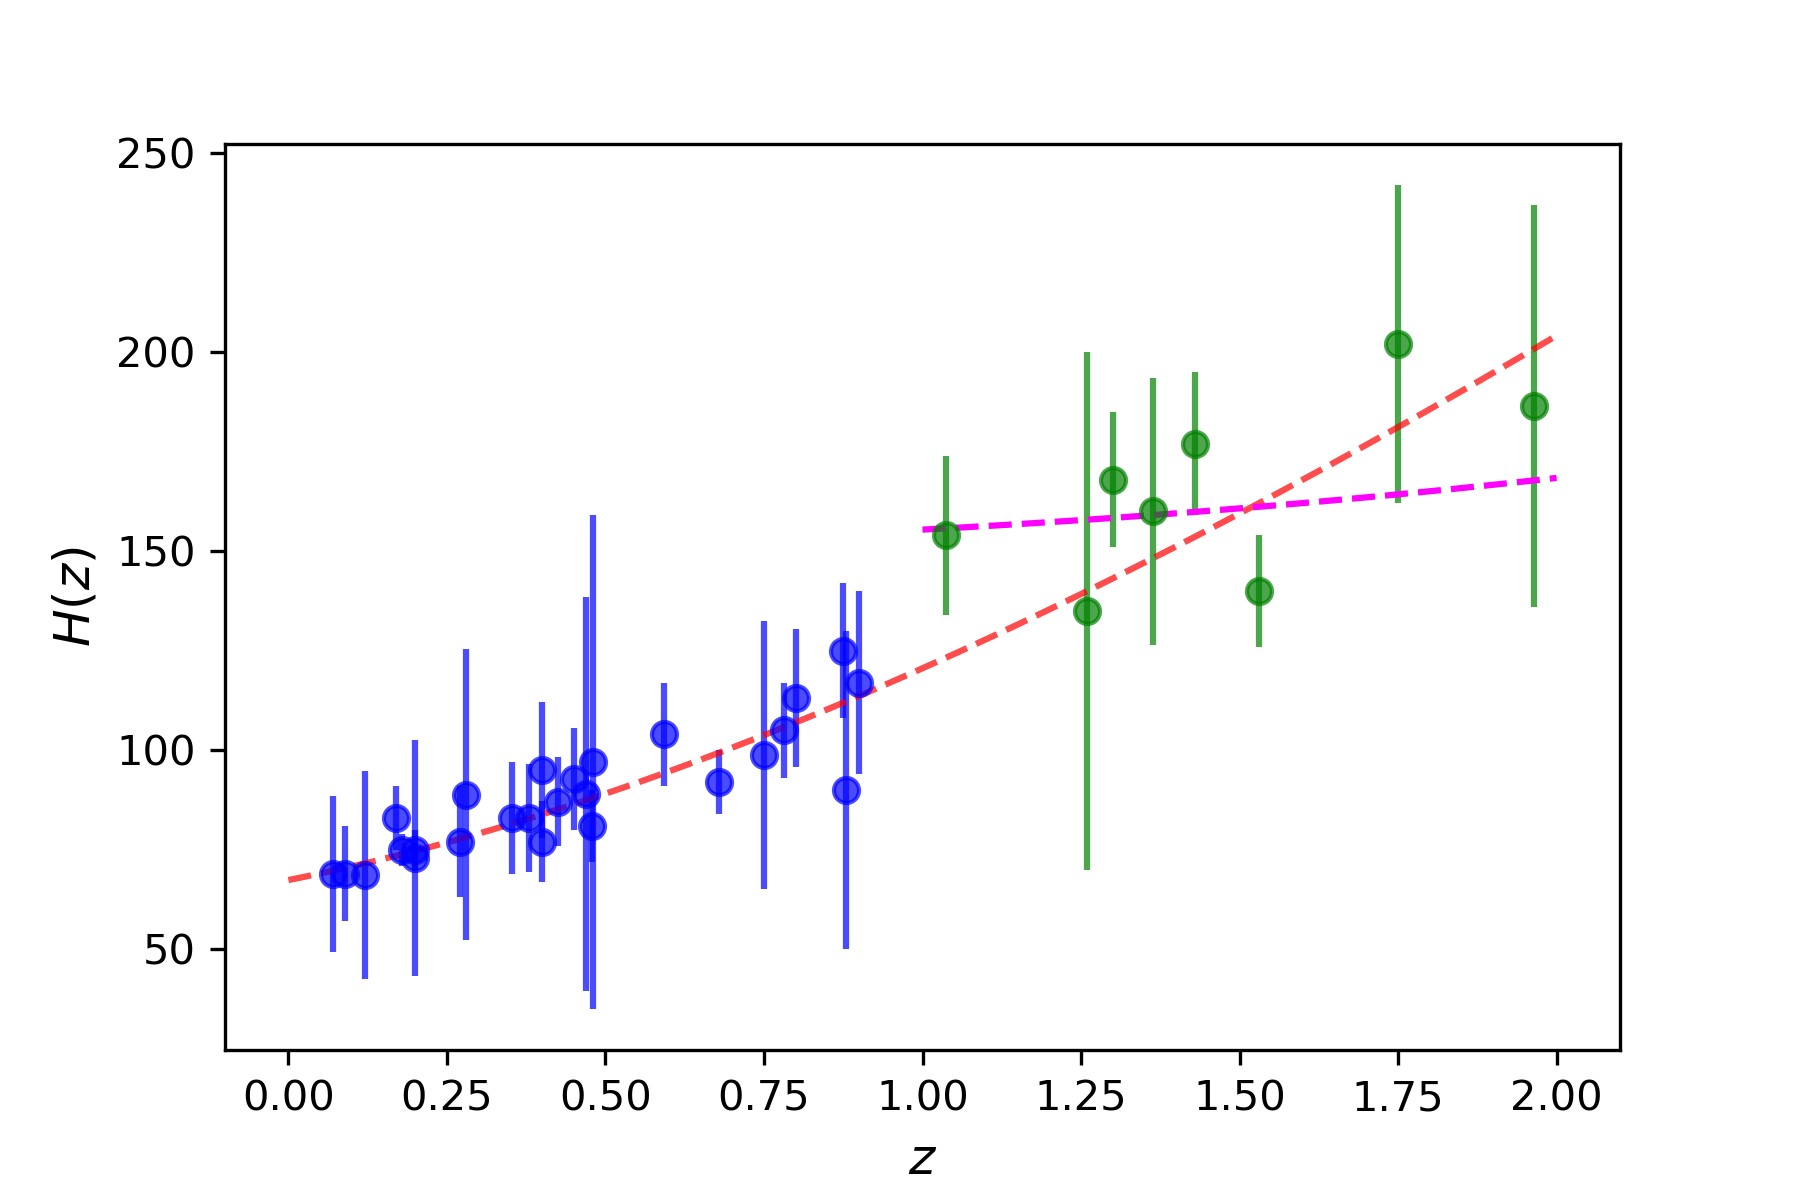
\includegraphics[width=120mm]{pressureless_matter/CCdata.png}
\caption{The CC data split above and below $z=1$ alongside the Planck-$\Lambda$CDM $H(z)$ (dashed red) and best fit $H(z)$ (dashed magenta) above $z=1$. From the high redshift data (green), it is evident that a horizontal $H(z)$ correspond to $\Omega_m =0$ should be preferred.}
\label{fig:CC} 
\end{figure}

\begin{figure}[htb]
   \centering
   \begin{tabular}{c}
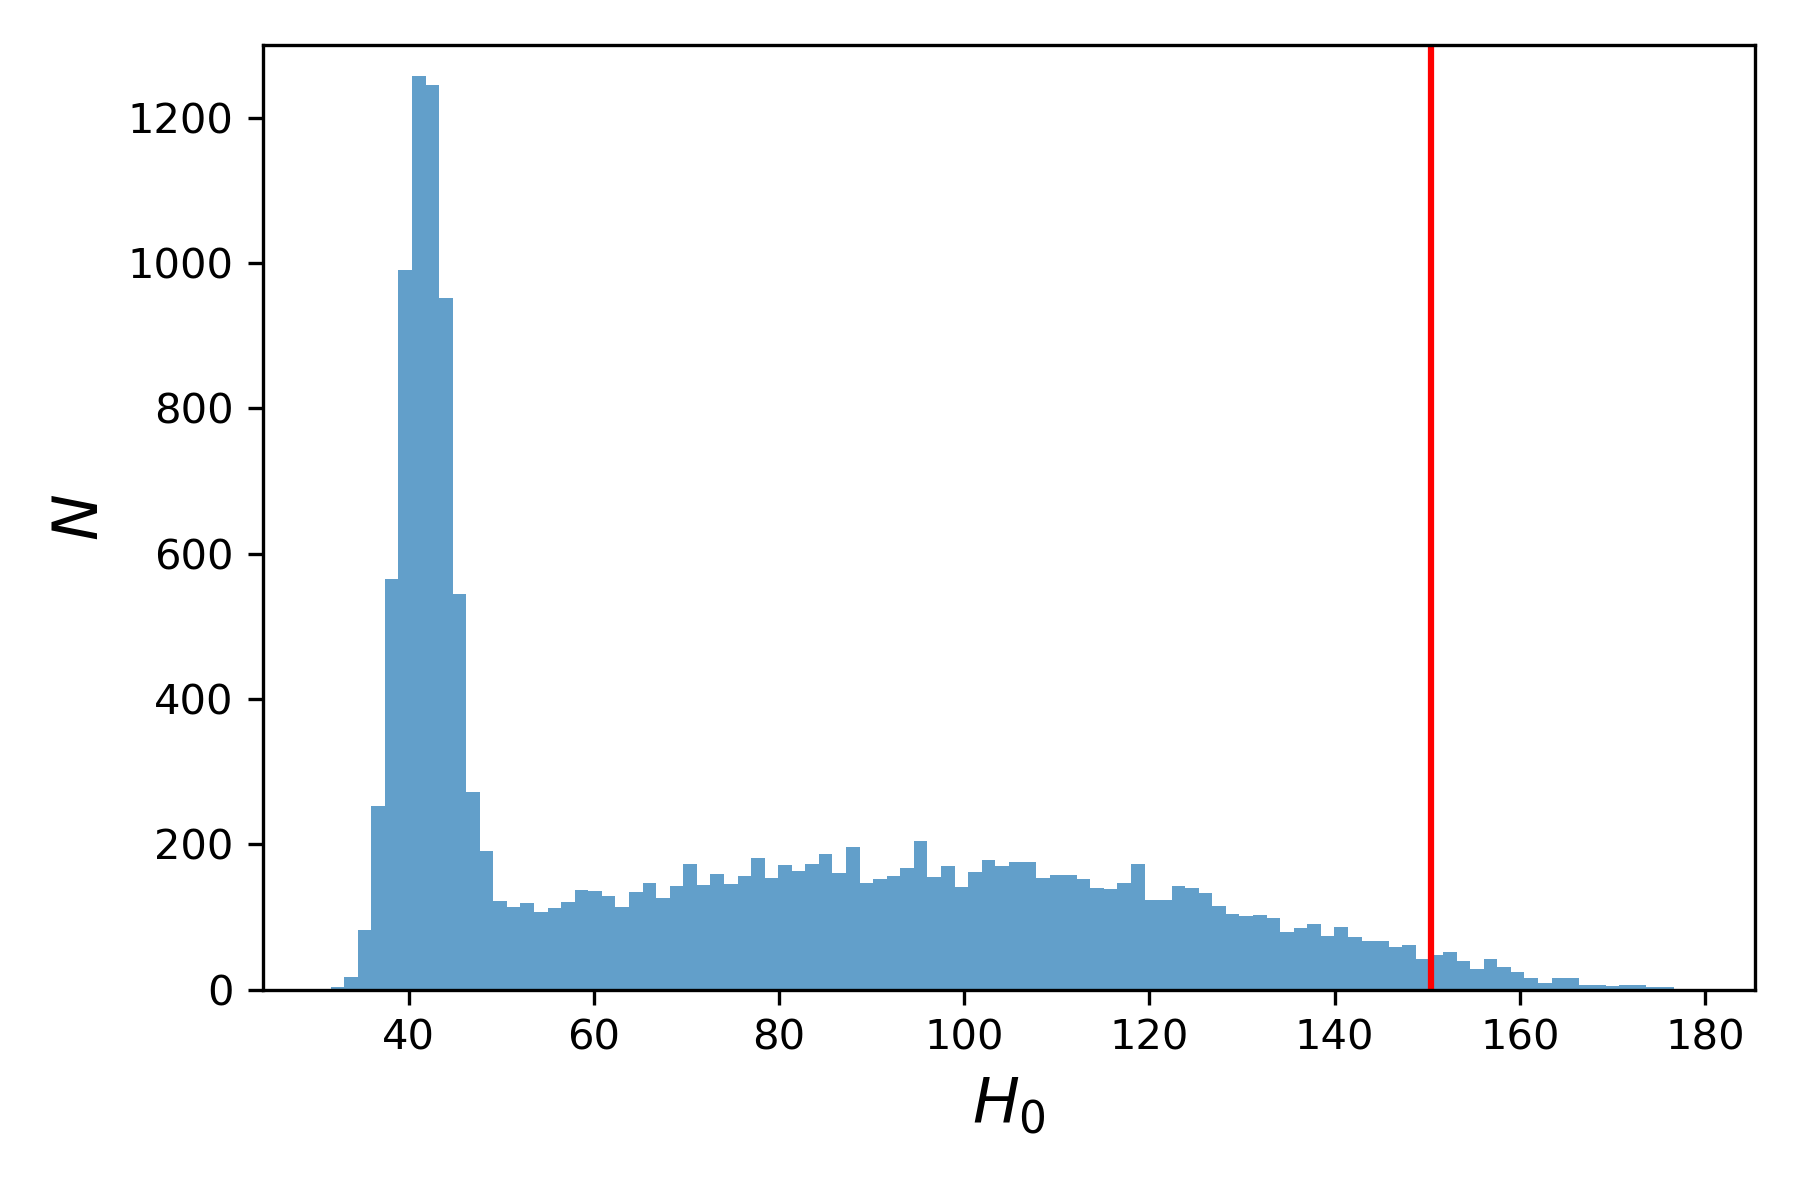
\includegraphics[width=100mm]{pressureless_matter/CC_h0_sim.png}  \\ 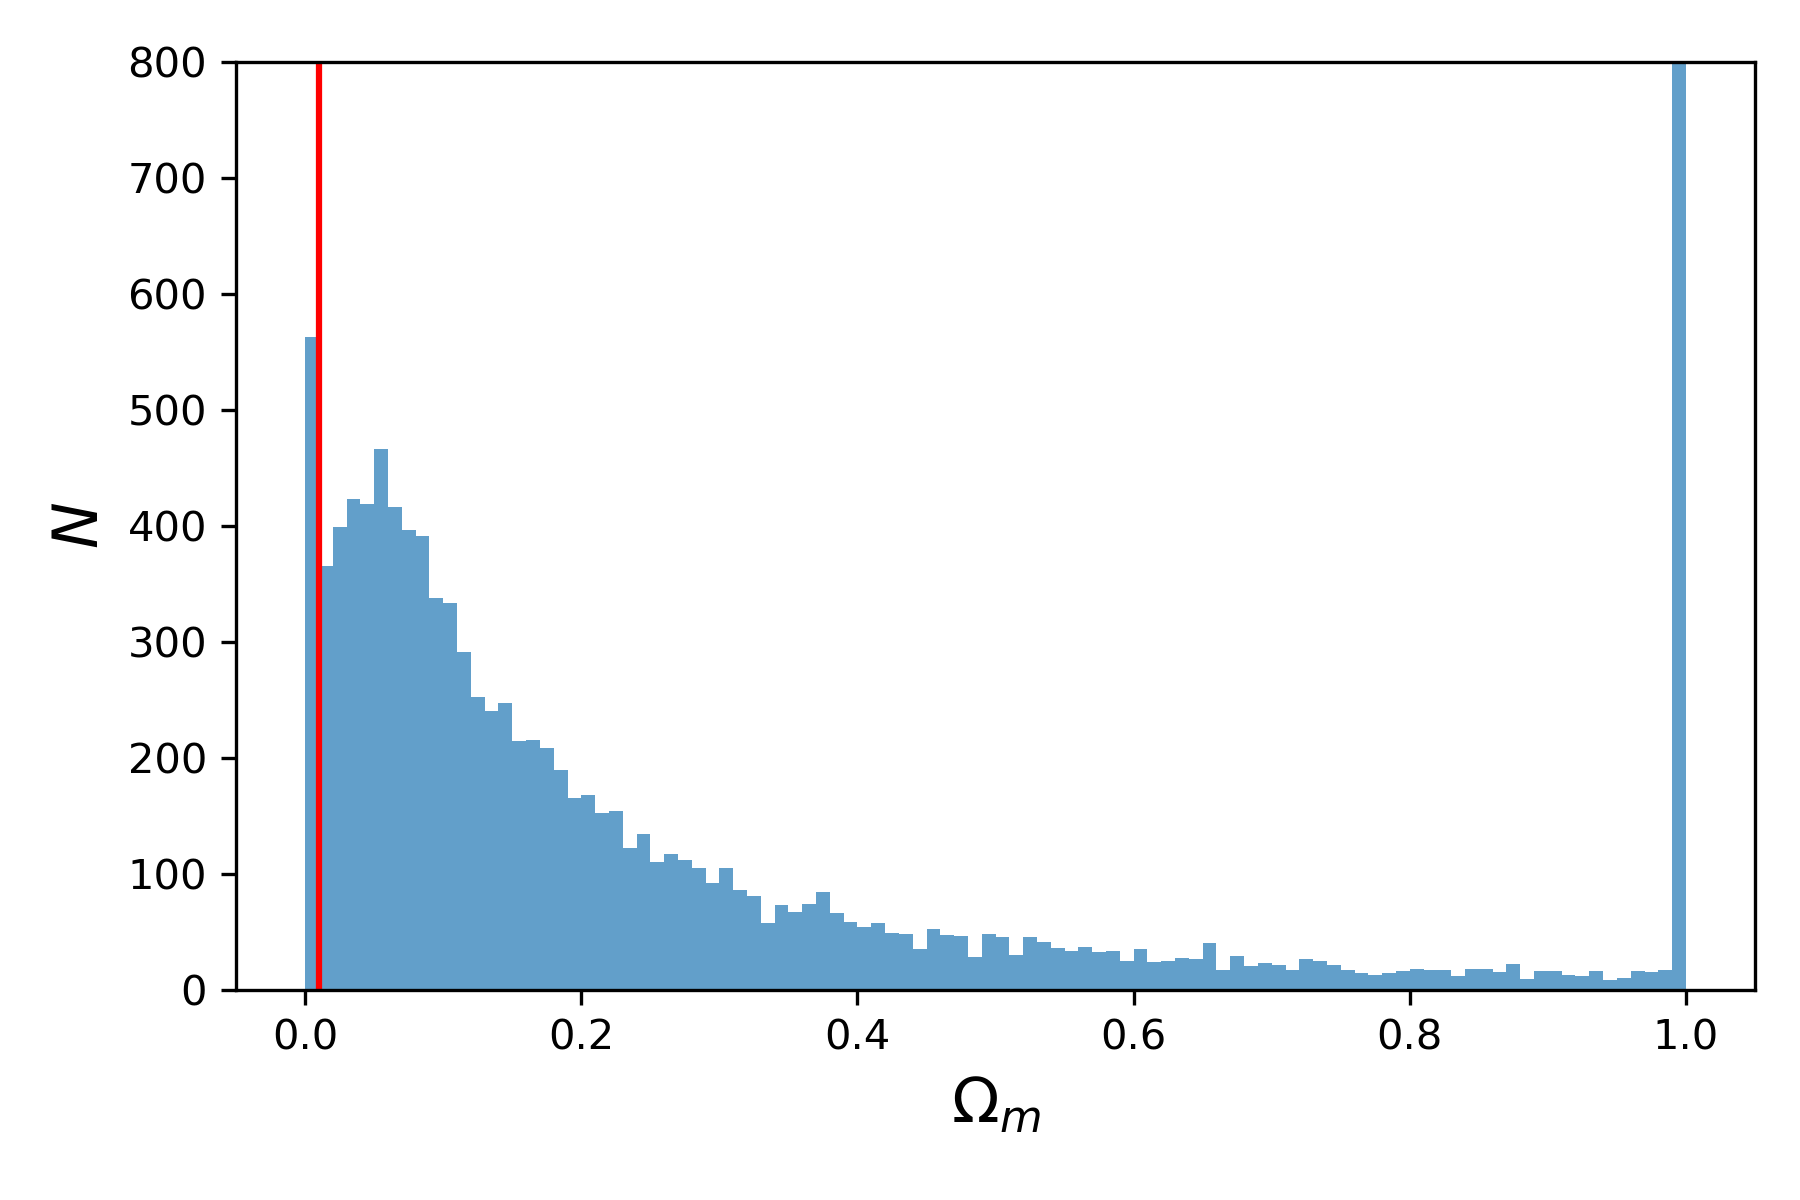
\includegraphics[width=100mm]{pressureless_matter/CC_om_sim.png}
    \end{tabular}
\caption{}
\label{fig:CCsims} 
\end{figure}

\begin{table}[htb]
    \centering
    \begin{tabular}{c|c|c|c|c|c}
    \rule{0pt}{3ex} $z_{\textrm{min}}$ & \# CC & \multicolumn{2}{c}{Fisher Matrix}  & \multicolumn{2}{|c}{MCMC} \\
    \hline
    \rule{0pt}{3ex} & & $H_0$ (km/s/Mpc) & $\Omega_m$ & $H_0$ (km/s/Mpc) & $\Omega_m$ \\
    \hline
    \rule{0pt}{3ex} $0$ & $34$ & $68.14 \pm 3.07$ & $0.320 \pm 0.059$ & $67.76^{+3.03}_{-3.09}$  ($68.12$) & $0.328^{+0.065}_{-0.055}$ ($0.321$) \\
    \hline 
    \rule{0pt}{3ex} $0.2$ & $27$ & $65.03 \pm 6.65$ & $0.368 \pm 0.118$ & $63.05^{+6.64}_{-7.23}$ ($64.98$) & $0.405^{+0.170}_{-0.111}$ ($0.369$) \\
    \hline 
    \rule{0pt}{3ex} $0.4$ & $22$ & $62.42 \pm 8.38$ & $0.411 \pm 0.161$ & $59.54^{+8.30}_{-8.22}$ ($62.39$) & $0.470^{+0.229}_{-0.151}$ ($0.411$)\\
    \hline 
    \rule{0pt}{3ex} $0.6$ & $15$ & $59.83 \pm 17.21$ & $0.454 \pm 0.338$ & $56.45^{+13.16}_{-9.33}$ ($59.86$) & $0.526^{+0.288}_{-0.225}$ ($0.453$) \\
    \hline 
    \rule{0pt}{3ex} $0.7$ & $14$ & $79.11 \pm 19.40$ & $0.222 \pm 0.162$ & $67.59^{+19.19}_{-16.57}$ ($79.18$) & $0.344^{+0.344}_{-0.178}$ ($0.222$) \\
    \hline 
    \rule{0pt}{3ex} $0.8$ & $11$ & $103.97 \pm 24.94$ & $0.097 \pm 0.088$ & $82.43^{+28.33}_{-27.03}$ ($104.02$) & $0.206^{+0.357}_{-0.131}$ ($0.096$) \\
    \hline 
    \rule{0pt}{3ex} $1$ & $8$ & $150.37 \pm 31.21$ & $0.010 \pm 0.035$ & $108.92^{+33.94}_{-44.47}$ ($150.38$) & $0.087^{+0.304}_{-0.068}$ ($0.010$) \\
    \hline 
    \rule{0pt}{3ex} $1.2$ & $7$ & $154.35 \pm 42.95$ & $0.006 \pm 0.042$ & $83.07^{+48.52}_{-32.19}$ ($154.47$) & $0.194^{+0.439}_{-0.159}$ ($0.006$) \\
    \hline 
    \rule{0pt}{3ex} $1.4$ & $4$ & $125.41 \pm 79.55$ & $0.039 \pm 0.132$ & $65.25^{+46.52}_{-20.31}$ ($125.38$) & $0.320^{+0.429}_{-0.253}$ ($0.039$) \\
    \hline 
    \rule{0pt}{3ex} $1.5$ & $3$ & $36.12 \pm 72.69$ & $1.000 \pm 4.269$ & $55.00^{+34.66}_{-14.61}$ ($36.12$) & $0.320^{+0.429}_{-0.253}$ ($0.999$)
    \end{tabular}
    \caption{\red{The expressions in brackets are the $(H_0, \Omega_m)$ values that minimise the $\chi^2$ from the MCMC chain.}}
    \label{tab:LCDM_CC}
\end{table}

\begin{figure}[htb]
   \centering
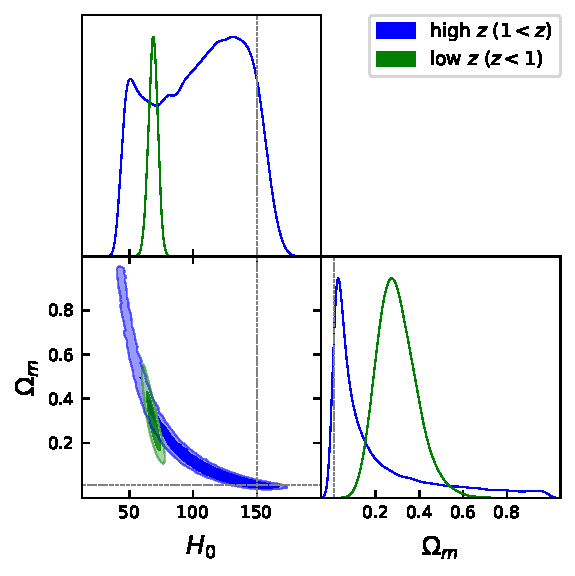
\includegraphics[width=100mm]{pressureless_matter/CC_zsplit1.pdf}
\caption{Cosmological parameter inferences from MCMC chains for the CC data split at $z=1$. Dashed lines denote the extremum of the $\chi^2$. For high redshift data, $\Omega_m$ is consistent with $\Omega_m = 0$, implying a constant Hubble parameter $H(z)=\textrm{constant} \sim 150$ km/s/Mpc. The secondary peak evident in the $H_0$ posterior arises from projecting the long tails in the $\Omega_m$ posterior onto the $H_0$ axis. The dashed lines correspond to the best fit parameters of the high z sample $(H_0, \Omega_m) = (150.37, 0.0098)$. This agrees well with the minimum $\chi^2$ from the MCMC chain, $(H_0, \Omega_m) = (150.27,0.0099)$.}
\label{fig:CCsplit1} 
\end{figure}

We clearly see some puzzling results in Table \ref{tab:LCDM_CC}, whereby MCMC marginalisation leads to 1 $\sigma$ confidence intervals that do not contain the best fit values, i. e. the values corresponding to the extremum of the $chi^2$. Nevertheless, when we run the MCMC chain through the $\chi^2$ and isolate the minimum value across the entire chain, we see that this is consistent with the best fit. It should be stressed that binning $H(z)$ constraints leads to non-Gaussian probability density functions (PDFs) when one fits exclusively high redshift mock data \cite{Colgain:2022tql}, so it may be expected that MCMC marginalisation returns unexpected results. To counteract this, we follow \cite{Gomez-Valent:2022hkb} and turn to profile distributions (PD). The basic idea is to study the ratio 
\be
R(\theta_1) = \frac{\tilde{P}(\theta_1)}{\max_{\theta_1} \tilde{P}(\theta_1) },  
\ee
where $\tilde{P}(\theta_1)$ is the PD for $\theta_1$ of a normalised distribution $P(\theta_1, \theta_2)$ with parameter sets $\theta_1$ and $\theta_2$. In other words, $\tilde{P}(\theta_1)$ is the maximum of $P$ for each $\theta_1$ along the directions of $\theta_2$: 
\be
\label{PD}
\tilde{P} (\theta_1) = \max_{\theta_2} P(\theta_1, \theta_2). 
\ee
We can be much more explicit. Consider the probability 
\be
P(\theta_1, \theta_2) = \exp \left( - \frac{1}{2} \chi^2(\theta_1, \theta_2) \right), 
\ee
where $\theta_1 = H_0$ and $\theta_2 = \Omega_m$, as in our case of interest. The maximum value of $P$ occurs for the minimum value of $\chi^2$, $P_{\textrm{max}} = e^{-\frac{1}{2} \chi^2_{\textrm{min}}}$. In this concrete setting, the PD becomes 
\be
\tilde{P}(\theta_1) = e^{-\frac{1}{2} \chi^2_{\textrm{min}}(\theta_1)}, 
\ee
where $\chi^2_{\textrm{min}}(\theta_1)$ denotes the minimum value of the $\chi^2$ along the $\theta_2$ direction for a fixed $\theta_1$ value. In practice, one can extract this information from the MCMC chain by breaking the $\theta_1$ direction up into bins and finding the minimum of the $\chi^2$ for each entry in the MCMC chain in that particular bin. Having done so, we are in a position to define a probability density function \cite{Gomez-Valent:2022hkb}: 
\be
\label{w}
w(\theta_1) = \frac{e^{-\frac{1}{2} \chi^2_{\textrm{min}}(\theta_1)}}{\int e^{-\frac{1}{2} \chi^2_{\textrm{min}}(\theta_1)} \dd \theta_1} = \frac{R(\theta_1)}{\int R(\theta_1) \dd \theta_1}, 
\ee
where in the second equality we have divided top and bottom by $P_{\textrm{max}} = e^{-\frac{1}{2} \chi^2_{\textrm{min}}}$. Note that $\int_{-\infty}^{+\infty} w(\theta_1) \dd \theta_1 = 1$ by construction, so $w(\theta_1)$ describes a normalised PDF. For this reason, we can identify the $1 \sigma$ confidence interval corresponding to the 68\% confidence level by simply identify $\theta_1^{(1)}$ and $\theta_1^{(2)}$ such that \cite{Gomez-Valent:2022hkb}
\be
\label{w1sigma}
\int_{\theta_1^{(1)}}^{\theta_1^{(2)}} w(\theta_1) \dd \theta_1 = 0.68, \quad w(\theta_1) = w(\theta_2). 
\ee
We will outline how this can be simply done when we turn to an explicit example. 

Our first port of call is employing the PD methodology to a redshift range where distributions are Gaussian, as is evident from the agreement between the peak of the posteriors and the best fit values of $(H_0, \Omega_m)$. For this reason, we focus on the first entry in Table \ref{tab:LCDM_CC}. Our first objective is to recover errors in the Gaussian regime where both MCMC marginalisation works well. This provides a consistency check on the PD methodology. 

We start by running a long MCMC chain and begin by analysing $H_0$. From the chain we identify the smallest and largest value of $H_0$ in the chain and break up this range into approximately 100 uniform bins, which we label using the $H_0$ value at the centre of the bin. In each $H_0$ bin we identify the minimum value of the $\chi^2$, $\chi^2_{\textrm{min}}(H_0)$, and calculate $R(H_0) = e^{-\frac{1}{2} \Delta \chi^2 (H_0)}$ in each bin, where we have defined $\Delta \chi_{\textrm{min}}^2 (H_0) : = \chi^2_{\textrm{min}}(H_0) - \chi^2_{\textrm{min}}$. Here, we stress again that $\chi^2_{\textrm{min}}$ is the minimum $\chi^2$ for the entire MCMC chain, essentially corresponding to the best fit values, whereas $\chi^2_{\textrm{min}} (H_0)$ is only the minimum at a fixed $H_0$ value for a particular bin. By construction, $R(H_0)$ is a distribution peaked at $R(H_0) = 1$. In Fig. \ref{fig:H0_R_zmin0} we plot $R(H_0)$ against $H_0$. Since the $H_0$ distribution from the MCMC chain may be sparse in the tails of the distribution, we simply omit any empty bins. These missing data points are evident at lower values of $H_0$ in Fig. \ref{fig:H0_R_zmin0}. Nevertheless, with 100 bins, minus any empty bins, we have sufficient density of points to calculate the area under the $R(H_0)$ curve using Simpson's rule. Dividing $R(H_0)$ through by the result ensures that $R(H_0)$ is normalised as required by (\ref{w}). It is now easy to solve (\ref{w1sigma}) by simply imposing a threshold $\kappa$ and retaining only $R(H_0)$ and their corresponding $H_0$ values with a value larger than the threshold. Reducing the threshold one retains more and more of the $R(H_0)$ distribution starting from its peak. One terminates the process when the normalised area under the curve is $0.68$. One can improve the results by increasing the number of $H_0$ bins, if required. Working with the precision afforded to us by approximately 100 bins, the $1 \sigma$ confidence interval is $64.9 \leq H_0 \leq 71.3$ km/s/Mpc with a peak at the global minimum of the $\chi^2$ of $H_0 = 68.2$ km/s/Mpc. Thus, we get the following result, $H_0 = 68.2^{+3.1}_{-3.3}$ km/s/Mpc, which agrees well with the MCMC marginalisation result from the first entry in Table \ref{tab:LCDM_CC}. It is easy to repeat the steps with $\Omega_m$ to get $\Omega_m = 0.320^{+0.064}_{-0.056}$, and confirm that despite a meagre 100 odd bins, we recover results comparable with MCMC, in particular a mild non-Gaussianity is evident in the errors.

We now come to the meat and we transport ourselves into a regime where MCMC marginalisation leads to biased results. Concretely, we restrict ourselves to the eight data points in the range $1 < z < 2$. Once again, we start by performing an MCMC exploration of parameter space, before binning the chains in 200 odd bins to reconstruct $R(H_0)$ and $R(\Omega_m)$ in Fig. (). 

\begin{figure}[htb]
   \centering
   \begin{tabular}{cc}
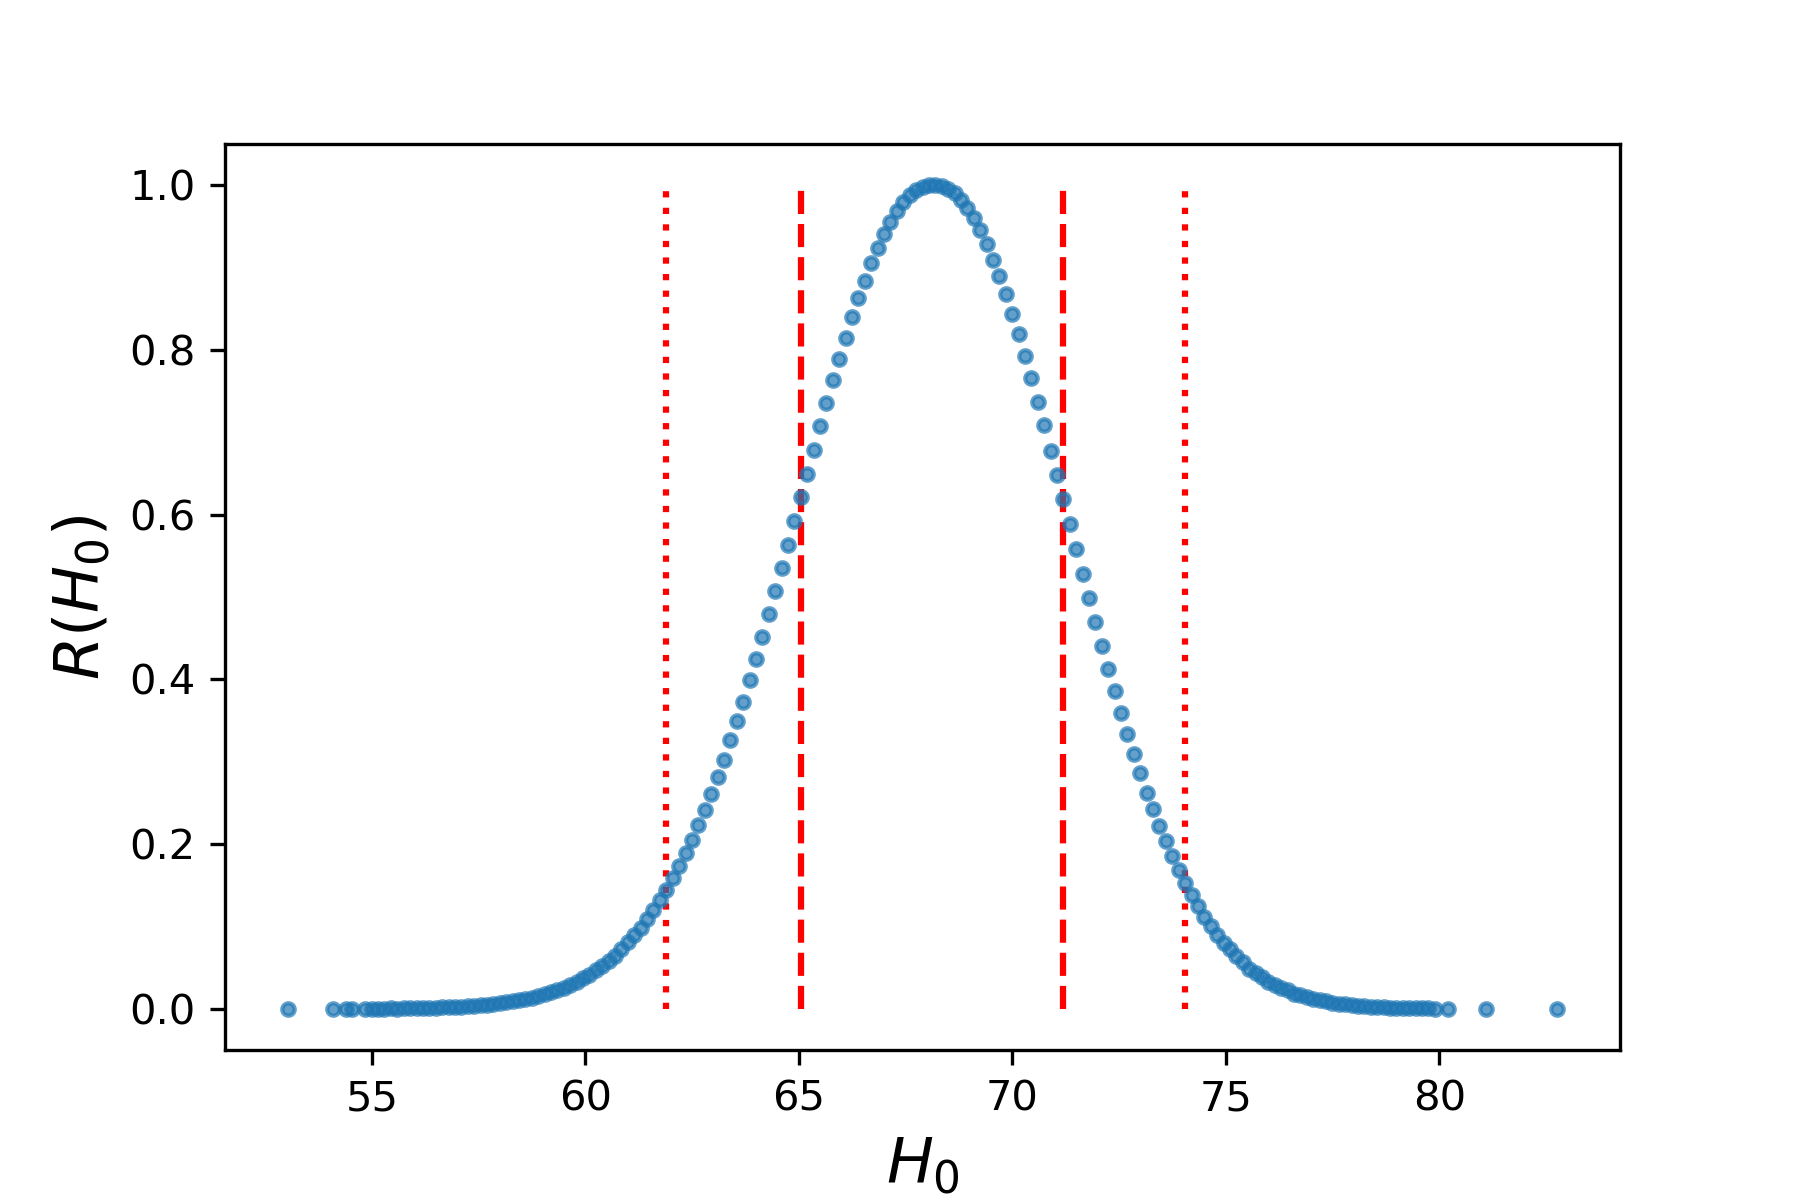
\includegraphics[width=80mm] {pressureless_matter/H0_R_zmin0.png} & 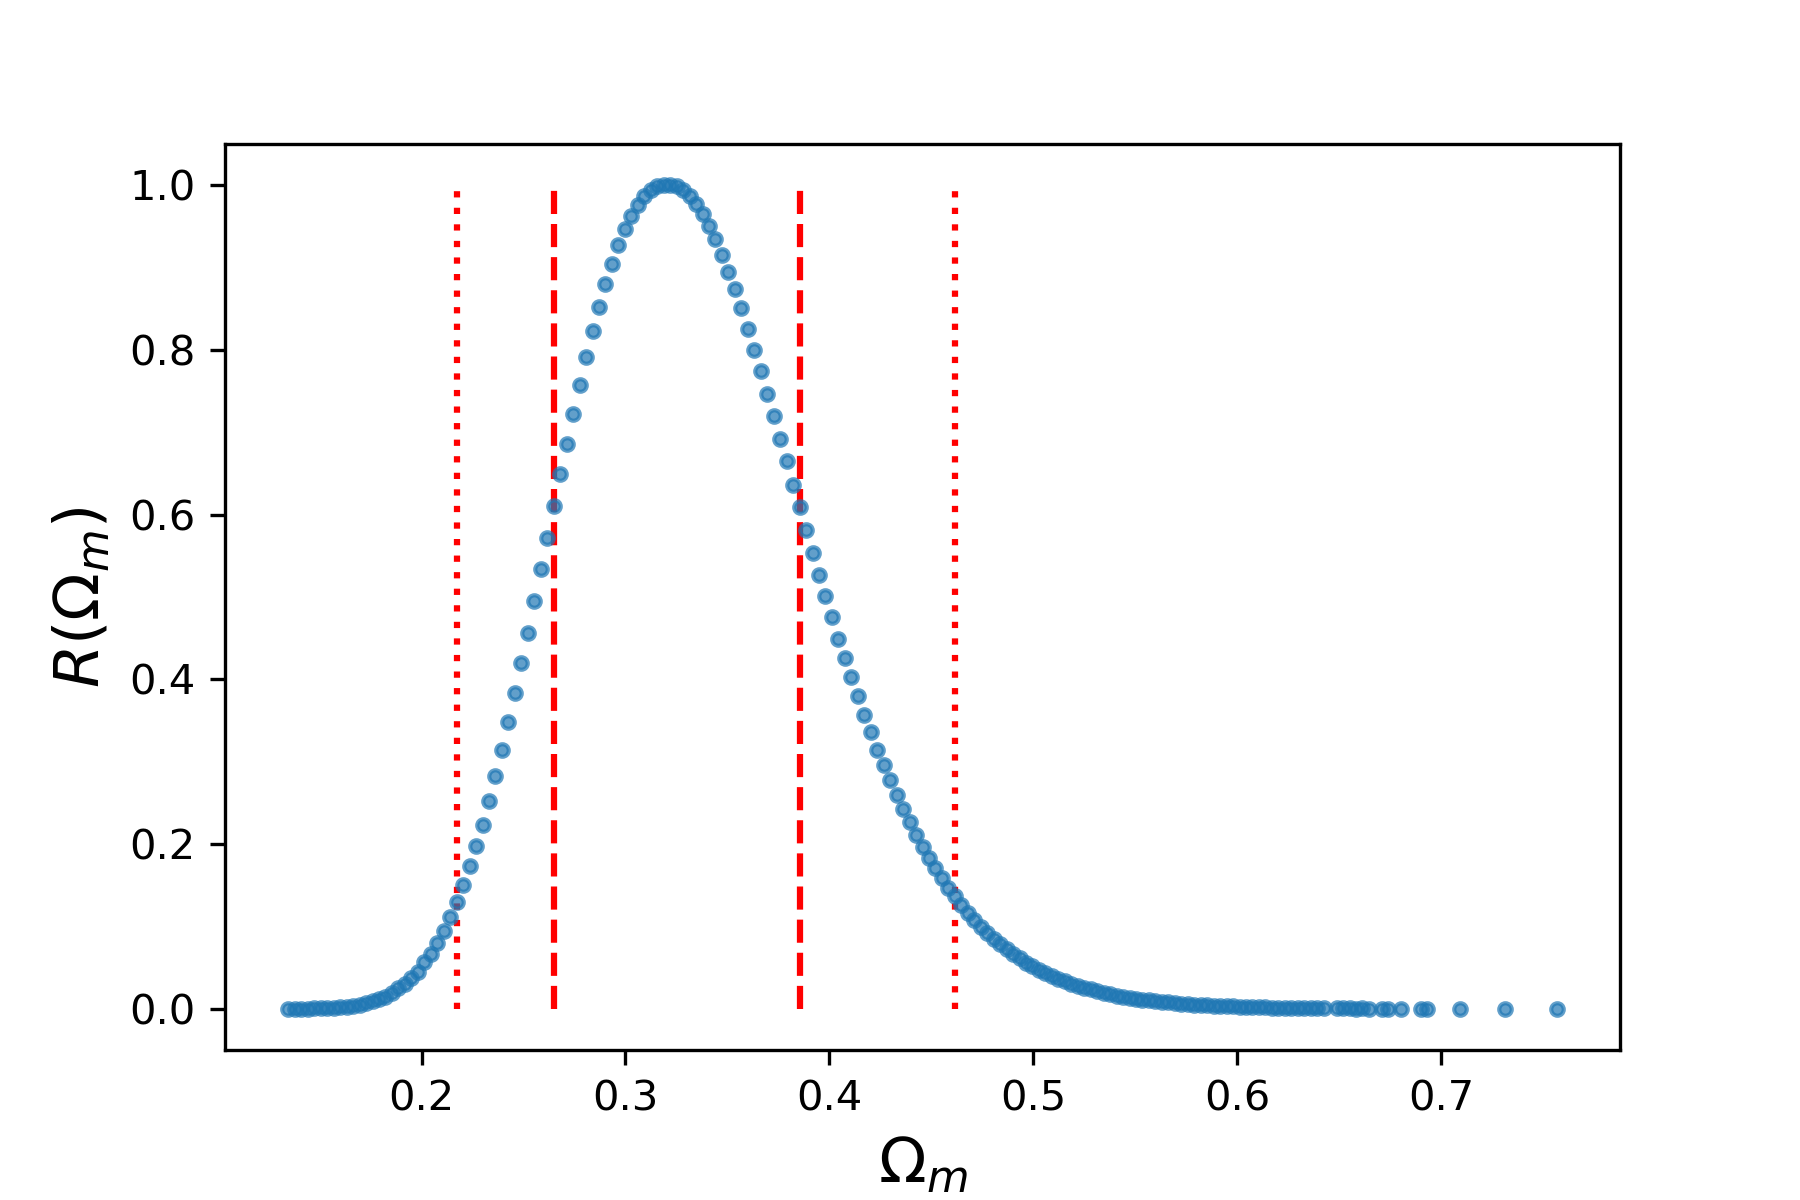
\includegraphics[width=80mm] {pressureless_matter/om_R_zmin0.png}
\end{tabular}
\caption{The dashed and dotted lines denote $1 \sigma$ and $2 \sigma$ confidence intervals.}
\label{fig:R_zmin0}
\end{figure}

\begin{table}[htb]
    \centering
    \begin{tabular}{c|c|c|c}
    \rule{0pt}{3ex} $z_{\textrm{min}}$ & \# CC & \multicolumn{2}{c}{PD}  \\
    \hline
    \rule{0pt}{3ex} & & $H_0$ (km/s/Mpc) & $\Omega_m$ \\
    \hline
    \rule{0pt}{3ex} $0$ & $34$ & $68.15^{+3.04}_{-3.11}$ & $0.320^{+0.065}_{-0.055}$ \\
    \hline 
    \rule{0pt}{3ex} $0.2$ & $27$ & $65.03^{+6.52}_{-7.03}$ & $0.368^{+0.167}_{-0.110}$ \\
    \hline 
    \rule{0pt}{3ex} $0.4$ & $22$ & $62.42^{+7.78}_{-8.74}$ & $0.411^{+0.236}_{-0.113}$ \\
    \hline
    \rule{0pt}{3ex} $0.6$ & $15$ & $59.75^{+11.73}_{-13.97}$ & $0.455^{+0.355}_{-0.160}$ \\
    \hline
    \rule{0pt}{3ex} $0.7$ & $14$ & $79.10^{+16.42}_{-20.56}$ & $0.222^{+0.386}_{-0.117}$ \\
    \hline
    \rule{0pt}{3ex} $0.8$ & $11$ & $103.94^{+22.88}_{-28.54}$ & $0.097^{+0.378}_{-0.074}$ \\
    \hline
    \rule{0pt}{3ex} $1$ & $8$ & $150.35^{+17.12}_{-35.95}$ & $ < 0.339$ \\
    \hline
    \rule{0pt}{3ex} $1.2$ & $7$ & $154.26^{+14.88}_{-54.82}$ & $ < 0.570$ \\
    \hline
    \rule{0pt}{3ex} $1.4$ & $4$ & $124.81^{+35.38}_{-52.60}$ & $ < 0.661$ \\
    \hline
    \rule{0pt}{3ex} $1.5$ & $3$ & $36.11^{+72.87}_{-2.43}$ & $ > 0.354$
    \end{tabular}
    \caption{\red{Fill out the rest of the table.}}
    \label{tab:LCDM_CC}
\end{table}


\begin{figure}[htb]
   \centering
   \begin{tabular}{cc}
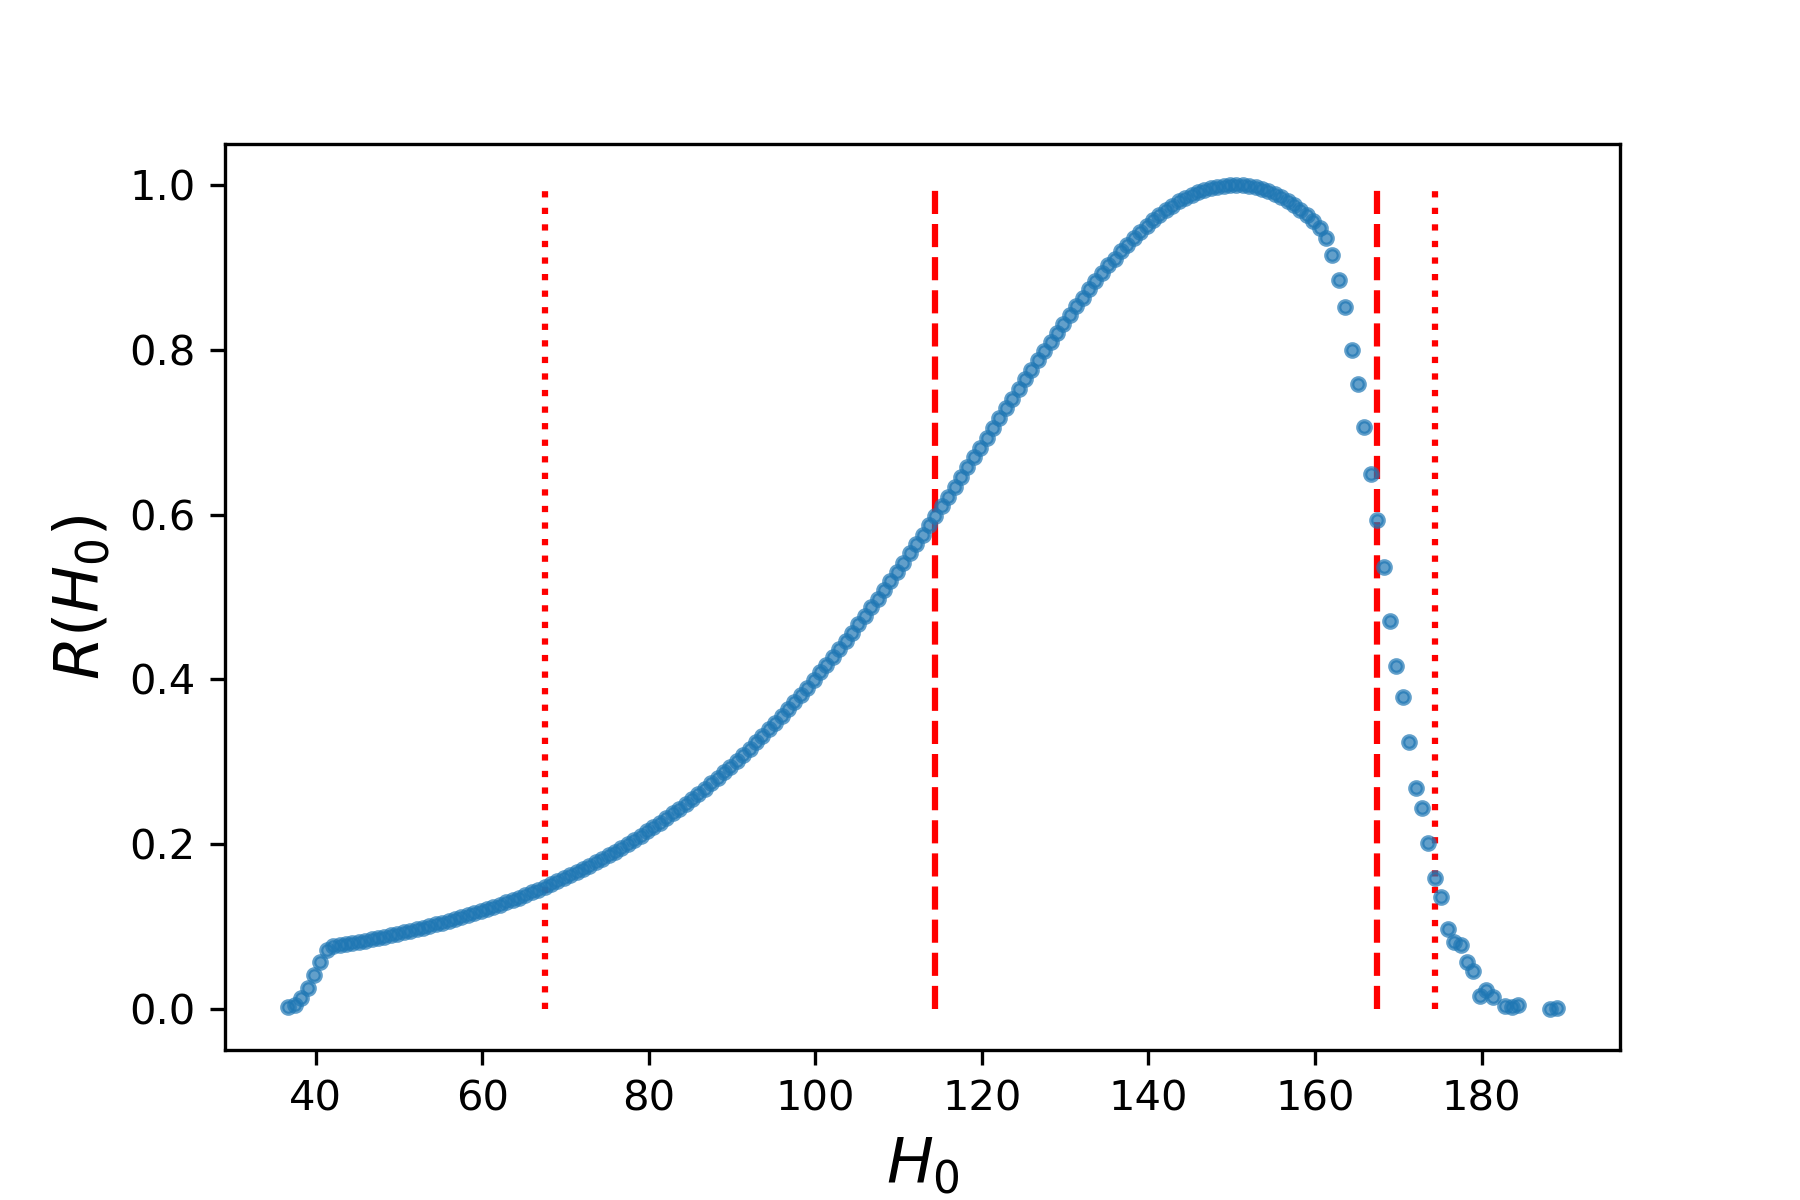
\includegraphics[width=80mm] {pressureless_matter/H0_R_zmin1.png} & 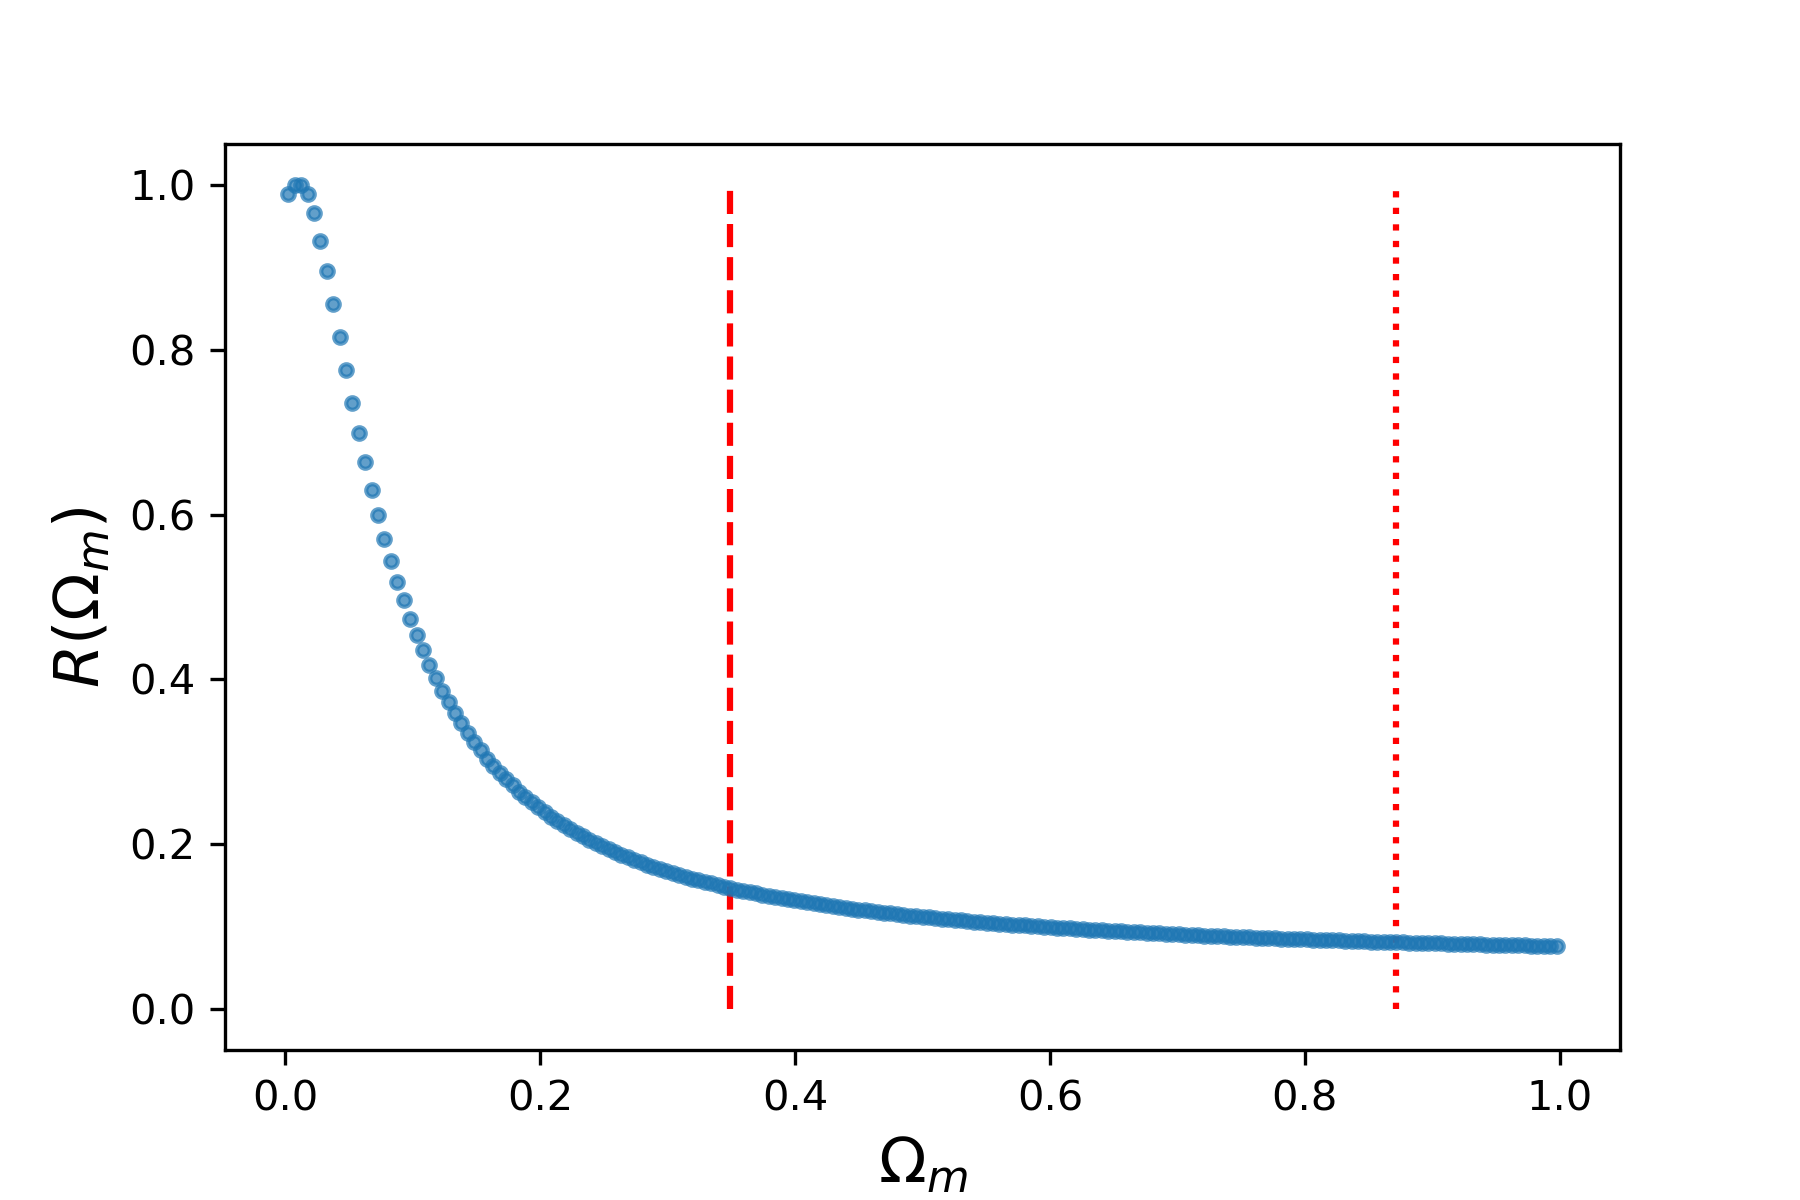
\includegraphics[width=80mm] {pressureless_matter/om_R_zmin1.png}
\end{tabular}
\caption{The dashed and dotted lines denote $1 \sigma$ and $2 \sigma$ confidence intervals.}
\label{fig:R_zmin1} 
\end{figure}

\appendix 

\section{Calculating a Fisher Matrix}
Consider the $\chi^2$
\be
\chi^2 = Q^{T} \cdot C^{-1} \cdot Q, 
\ee
where $C$ is the covariance matrix, which is simply the square of the $H_i$ errors on the diagonal and $Q$ is the vector, 
\be
Q_i = H_i - H_{\textrm{model}}(z_i), 
\ee
where $H_i$ is the y-data and $z_i$ is x-the data. Defining $H_{\textrm{model}}(z) = H_0 \sqrt{1-\Omega_m + \Omega_m (1+z)^3}$, we can now work out the derivatives
\bea
\partial_{H_0} Q_i &=& -\sqrt{1-\Omega_m + \Omega_m (1+z_i)^3}, \quad  \partial_{\Omega_m} Q_i = - \frac{1}{2} H_0 (z_i^3 + 3 z_i^2 + 3 z_i)/\sqrt{1-\Omega_m + \Omega_m (1+z_i)^3} \nn 
\partial^2_{H_0} Q_i &=& 0, \quad
\partial_{H_0} \partial_{\Omega_m} Q_i = - \frac{1}{2} (z_i^3 + 3 z_i^2 + 3 z_i)/\sqrt{1-\Omega_m + \Omega_m (1+z_i)^3}, \\
\partial^2_{\Omega_m} Q_i &=& \frac{1}{4} H_0 (z_i^3 + 3 z_i^2 + 3 z_i)^2/(1-\Omega_m + \Omega_m (1+z_i)^3)^{\frac{3}{2}}. 
\eea

We can then define the Fisher matrix 
\be
F_{ij} = \frac{1}{2} \frac{\partial^2 \chi^2(H_0, \Omega_m)}{\partial p_i \partial p_j}
\ee
where $p_i \in \{ H_0, \Omega_m \}$.Note that the Fisher matrix is evaluated on the best fit parameters. The result is a $2 \times 2$ matrix, which one inverts and the estimated errors are the square root of the diagonal entries. 

The introduction of a Planck prior leads to the addition of the term 
\be
\chi_{\textrm{prior}}^2 = \frac{(\Omega_m h^2 - 0.1430)^2}{(0.0011)^2}, 
\ee
where we recall that $h = H_0/100$. 


\begin{thebibliography}{99}

\bibitem{Scolnic:2021amr}
D.~Scolnic, D.~Brout, A.~Carr, A.~G.~Riess, T.~M.~Davis, A.~Dwomoh, D.~O.~Jones, N.~Ali, P.~Charvu and R.~Chen, \textit{et al.}
%``The Pantheon+ Analysis: The Full Data Set and Light-curve Release,''
Astrophys. J. \textbf{938} (2022) no.2, 113
%doi:10.3847/1538-4357/ac8b7a
[arXiv:2112.03863 [astro-ph.CO]].
%123 citations counted in INSPIRE as of 28 Jun 2023


\bibitem{Brout:2022vxf}
D.~Brout, D.~Scolnic, B.~Popovic, A.~G.~Riess, J.~Zuntz, R.~Kessler, A.~Carr, T.~M.~Davis, S.~Hinton and D.~Jones, \textit{et al.}
%``The Pantheon+ Analysis: Cosmological Constraints,''
Astrophys. J. \textbf{938} (2022) no.2, 110
%doi:10.3847/1538-4357/ac8e04
[arXiv:2202.04077 [astro-ph.CO]].
%194 citations counted in INSPIRE as of 28 Jun 2023


\bibitem{Malekjani:2023dky}
M.~Malekjani, R.~M.~Conville, E.~\'O.~Colg\'ain, S.~Pourojaghi and M.~M.~Sheikh-Jabbari,
%``Negative Dark Energy Density from High Redshift Pantheon+ Supernovae,''
[arXiv:2301.12725 [astro-ph.CO]].
%13 citations counted in INSPIRE as of 28 Jun 2023


\bibitem{Colgain:2022tql}
E.~\'O~Colg\'ain, M.~M.~Sheikh-Jabbari and R.~Solomon,
%``High redshift \ensuremath{\Lambda}CDM cosmology: To bin or not to bin?,''
Phys. Dark Univ. \textbf{40} (2023), 101216
%doi:10.1016/j.dark.2023.101216
[arXiv:2211.02129 [astro-ph.CO]].
%10 citations counted in INSPIRE as of 28 Jun 2023

\bibitem{Hou:2020rse}
J.~Hou, A.~G.~S\'anchez, A.~J.~Ross, A.~Smith, R.~Neveux, J.~Bautista, E.~Burtin, C.~Zhao, R.~Scoccimarro and K.~S.~Dawson, \textit{et al.}
%``The Completed SDSS-IV extended Baryon Oscillation Spectroscopic Survey: BAO and RSD measurements from anisotropic clustering analysis of the Quasar Sample in configuration space between redshift 0.8 and 2.2,''
Mon. Not. Roy. Astron. Soc. \textbf{500} (2020) no.1, 1201-1221
%:10.1093/mnras/staa3234
[arXiv:2007.08998 [astro-ph.CO]].
%135 citations counted in INSPIRE as of 28 Jun 2023

\bibitem{Neveux:2020voa}
R.~Neveux, E.~Burtin, A.~de Mattia, A.~Smith, A.~J.~Ross, J.~Hou, J.~Bautista, J.~Brinkmann, C.~H.~Chuang and K.~S.~Dawson, \textit{et al.}
%``The completed SDSS-IV extended Baryon Oscillation Spectroscopic Survey: BAO and RSD measurements from the anisotropic power spectrum of the quasar sample between redshift 0.8 and 2.2,''
Mon. Not. Roy. Astron. Soc. \textbf{499} (2020) no.1, 210-229
%doi:10.1093/mnras/staa2780
[arXiv:2007.08999 [astro-ph.CO]].
%133 citations counted in INSPIRE as of 28 Jun 2023

\bibitem{duMasdesBourboux:2020pck}
H.~du Mas des Bourboux, J.~Rich, A.~Font-Ribera, V.~de Sainte Agathe, J.~Farr, T.~Etourneau, J.~M.~Le Goff, A.~Cuceu, C.~Balland and J.~E.~Bautista, \textit{et al.}
%``The Completed SDSS-IV Extended Baryon Oscillation Spectroscopic Survey: Baryon Acoustic Oscillations with Ly\ensuremath{\alpha} Forests,''
Astrophys. J. \textbf{901} (2020) no.2, 153
%doi:10.3847/1538-4357/abb085
[arXiv:2007.08995 [astro-ph.CO]].
%172 citations counted in INSPIRE as of 28 Jun 2023

\bibitem{Jimenez:2001gg}
R.~Jimenez and A.~Loeb,
%``Constraining cosmological parameters based on relative galaxy ages,''
Astrophys. J. \textbf{573} (2002), 37-42
%doi:10.1086/340549
[arXiv:astro-ph/0106145 [astro-ph]].
%598 citations counted in INSPIRE as of 28 Jun 2023

\bibitem{Jimenez:2023flo}
R.~Jimenez, M.~Moresco, L.~Verde and B.~D.~Wandelt,
%``Cosmic Chronometers with Photometry: a new path to $H(z)$,''
[arXiv:2306.11425 [astro-ph.CO]].
%0 citations counted in INSPIRE as of 28 Jun 2023

\bibitem{Tomasetti:2023kek}
E.~Tomasetti, M.~Moresco, N.~Borghi, K.~Jiao, A.~Cimatti, L.~Pozzetti, A.~C.~Carnall, R.~J.~McLure and L.~Pentericci,
%``A new measurement of the expansion history of the Universe at z=1.26 with cosmic chronometers in VANDELS,''
[arXiv:2305.16387 [astro-ph.CO]].
%1 citations counted in INSPIRE as of 28 Jun 2023

\bibitem{Wong:2019kwg}
K.~C.~Wong, S.~H.~Suyu, G.~C.~F.~Chen, C.~E.~Rusu, M.~Millon, D.~Sluse, V.~Bonvin, C.~D.~Fassnacht, S.~Taubenberger and M.~W.~Auger, \textit{et al.}
``H0LiCOW \textendash{} XIII. A 2.4 per cent measurement of H0 from lensed quasars: 5.3\ensuremath{\sigma} tension between early- and late-Universe probes,''
Mon. Not. Roy. Astron. Soc. \textbf{498} (2020) no.1, 1420-1439
%doi:10.1093/mnras/stz3094
[arXiv:1907.04869 [astro-ph.CO]].
%804 citations counted in INSPIRE as of 18 May 2023

\bibitem{Millon:2019slk}
M.~Millon, A.~Galan, F.~Courbin, T.~Treu, S.~H.~Suyu, X.~Ding, S.~Birrer, G.~C.~F.~Chen, A.~J.~Shajib and D.~Sluse, \textit{et al.}
``TDCOSMO. I. An exploration of systematic uncertainties in the inference of $H_0$ from time-delay cosmography,''
Astron. Astrophys. \textbf{639} (2020), A101
%doi:10.1051/0004-6361/201937351
[arXiv:1912.08027 [astro-ph.CO]].
%114 citations counted in INSPIRE as of 18 May 2023

\bibitem{DES:2019fny}
A.~J.~Shajib \textit{et al.} [DES],
``STRIDES: a 3.9 per cent measurement of the Hubble constant from the strong lens system DES J0408\ensuremath{-}5354,''
Mon. Not. Roy. Astron. Soc. \textbf{494} (2020) no.4, 6072-6102
%doi:10.1093/mnras/staa828
[arXiv:1910.06306 [astro-ph.CO]].
%147 citations counted in INSPIRE as of 18 May 2023

\bibitem{Shajib:2023uig}
A.~J.~Shajib, P.~Mozumdar, G.~C.~F.~Chen, T.~Treu, M.~Cappellari, S.~Knabel, S.~H.~Suyu, V.~N.~Bennert, J.~A.~Frieman and D.~Sluse, \textit{et al.}
``TDCOSMO. XIII. Improved Hubble constant measurement from lensing time delays using spatially resolved stellar kinematics of the lens galaxy,''
Astron. Astrophys. \textbf{673} (2023), A9
%doi:10.1051/0004-6361/202345878
[arXiv:2301.02656 [astro-ph.CO]].
%3 citations counted in INSPIRE as of 18 May 2023

\bibitem{Birrer:2020tax}
S.~Birrer, A.~J.~Shajib, A.~Galan, M.~Millon, T.~Treu, A.~Agnello, M.~Auger, G.~C.~F.~Chen, L.~Christensen and T.~Collett, \textit{et al.}
``TDCOSMO - IV. Hierarchical time-delay cosmography \textendash{} joint inference of the Hubble constant and galaxy density profiles,''
Astron. Astrophys. \textbf{643} (2020), A165
%doi:10.1051/0004-6361/202038861
[arXiv:2007.02941 [astro-ph.CO]].
%223 citations counted in INSPIRE as of 18 May 2023

\bibitem{Kelly:2023mgv}
P.~L.~Kelly, S.~Rodney, T.~Treu, M.~Oguri, W.~Chen, A.~Zitrin, S.~Birrer, V.~Bonvin, L.~Dessart and J.~M.~Diego, \textit{et al.}
``Constraints on the Hubble constant from Supernova Refsdal's reappearance,''
%doi:10.1126/science.abh1322
[arXiv:2305.06367 [astro-ph.CO]].
%1 citations counted in INSPIRE as of 18 May 2023

\bibitem{DES:2017lgx}
H.~Lin \textit{et al.} [DES],
``Discovery of the Lensed Quasar System DES J0408-5354,''
Astrophys. J. Lett. \textbf{838} (2017) no.2, L15
%doi:10.3847/2041-8213/aa624e
[arXiv:1702.00072 [astro-ph.GA]].
%28 citations counted in INSPIRE as of 18 May 2023

 \bibitem{Kelly:2023wzm}
P.~L.~Kelly, S.~Rodney, T.~Treu, S.~Birrer, V.~Bonvin, L.~Dessart, R.~J.~Foley, A.~V.~Filippenko, D.~Gilman and S.~Jha, \textit{et al.}
``The Magnificent Five Images of Supernova Refsdal: Time Delay and Magnification Measurements,''
Astrophys. J. \textbf{948} (2023) no.2, 93
%doi:10.3847/1538-4357/ac4ccb
[arXiv:2305.06377 [astro-ph.CO]].
%1 citations counted in INSPIRE as of 18 May 2023

\bibitem{Tomasetti:2023kek}
E.~Tomasetti, M.~Moresco, N.~Borghi, K.~Jiao, A.~Cimatti, L.~Pozzetti, A.~C.~Carnall, R.~J.~McLure and L.~Pentericci,
%``A new measurement of the expansion history of the Universe at z=1.26 with cosmic chronometers in VANDELS,''
[arXiv:2305.16387 [astro-ph.CO]].
%0 citations counted in INSPIRE as of 16 Jun 202

\bibitem{Gomez-Valent:2018hwc}
A.~G\'omez-Valent and L.~Amendola,
%``$H_0$ from cosmic chronometers and Type Ia supernovae, with Gaussian Processes and the novel Weighted Polynomial Regression method,''
JCAP \textbf{04} (2018), 051
%doi:10.1088/1475-7516/2018/04/051
[arXiv:1802.01505 [astro-ph.CO]].
%173 citations counted in INSPIRE as of 16 Jun 2023

\bibitem{Haridasu:2018gqm}
B.~S.~Haridasu, V.~V.~Lukovi\'c, M.~Moresco and N.~Vittorio,
%``An improved model-independent assessment of the late-time cosmic expansion,''
JCAP \textbf{10} (2018), 015
%doi:10.1088/1475-7516/2018/10/015
[arXiv:1805.03595 [astro-ph.CO]].
%92 citations counted in INSPIRE as of 16 Jun 2023

\bibitem{Moresco:2022phi}
M.~Moresco, L.~Amati, L.~Amendola, S.~Birrer, J.~P.~Blakeslee, M.~Cantiello, A.~Cimatti, J.~Darling, M.~Della Valle and M.~Fishbach, \textit{et al.}
%``Unveiling the Universe with emerging cosmological probes,''
Living Rev. Rel. \textbf{25} (2022) no.1, 6
%doi:10.1007/s41114-022-00040-z
[arXiv:2201.07241 [astro-ph.CO]].
%71 citations counted in INSPIRE as of 16 Jun 2023


\bibitem{Risaliti:2015zla}
G.~Risaliti and E.~Lusso,
%``A Hubble Diagram for Quasars,''
Astrophys. J. \textbf{815} (2015), 33
%doi:10.1088/0004-637X/815/1/33
[arXiv:1505.07118 [astro-ph.CO]].
%146 citations counted in INSPIRE as of 16 Jun 2023

\bibitem{Risaliti:2018reu}
G.~Risaliti and E.~Lusso,
%``Cosmological constraints from the Hubble diagram of quasars at high redshifts,''
Nature Astron. \textbf{3} (2019) no.3, 272-277
%doi:10.1038/s41550-018-0657-z
[arXiv:1811.02590 [astro-ph.CO]].
%213 citations counted in INSPIRE as of 16 Jun 2023

\bibitem{Lusso:2020pdb}
E.~Lusso, G.~Risaliti, E.~Nardini, G.~Bargiacchi, M.~Benetti, S.~Bisogni, S.~Capozziello, F.~Civano, L.~Eggleston and M.~Elvis, \textit{et al.}
%``Quasars as standard candles III. Validation of a new sample for cosmological studies,''
Astron. Astrophys. \textbf{642} (2020), A150
%doi:10.1051/0004-6361/202038899
[arXiv:2008.08586 [astro-ph.GA]].
%79 citations counted in INSPIRE as of 16 Jun 2023

\bibitem{Planck:2018vyg}
N.~Aghanim \textit{et al.} [Planck],
%``Planck 2018 results. VI. Cosmological parameters,''
Astron. Astrophys. \textbf{641} (2020), A6
% doi:10.1051/0004-6361/201833910
[arXiv:1807.06209 [astro-ph.CO]].
%5639 citations counted in INSPIRE as of 10 Aug 2021

\bibitem{Gomez-Valent:2022hkb}
A.~G\'omez-Valent,
%``Fast test to assess the impact of marginalization in Monte~Carlo analyses and its application to cosmology,''
Phys. Rev. D \textbf{106} (2022) no.6, 063506
%doi:10.1103/PhysRevD.106.063506
[arXiv:2203.16285 [astro-ph.CO]].
%20 citations counted in INSPIRE as of 11 Jul 2023

\end{thebibliography}
\end{document}